\documentclass[../../main.tex]{subfiles}
\begin{document}

{\bf [解]}
楕円$\dfrac{x^2}{17}+\dfrac{y^2}{8}=1$の外部の点$P(a,b)$を考える．

楕円の接線のうち$y$軸並行なものは$x=\pm\sqrt{17}$のみである．この時直交する接線は$y=\pm\sqrt{8}$である．この時$P=(\pm\sqrt{17},\pm\sqrt{8})$である．そこで以下$a \neq \pm\sqrt{17}$で考える．

\begin{figure}[htb]
\begin{center}
\begin{tikzpicture}[scale=1.1, >=stealth]

  % --- 1. 幾何パラメータ (楕円・準円・点P) ---
  \pgfmathsetmacro{\ra}{sqrt(17)} % a = sqrt(17) ≒ 4.123
  \pgfmathsetmacro{\rb}{sqrt(8)}  % b = sqrt(8)  ≒ 2.828
  \pgfmathsetmacro{\R}{5}         % 準円半径 R = sqrt(17+8) = 5

  % 点 P(a, b) の例: P(3, 4)
  \def\Px{3.0}
  \def\Py{4.0}
  \coordinate (P) at (\Px, \Py);

  % 2本の接線の傾き m1, m2 (m^2 + 3m - 1 = 0 の解)
  \pgfmathsetmacro{\mOne}{(-3 + sqrt(13))/2} % m1 ≒  0.3028
  \pgfmathsetmacro{\mTwo}{(-3 - sqrt(13))/2} % m2 ≒ -3.3028

  % --- 2. 座標軸 ---
  \draw[->, thick] (-5.8, 0) -- (5.8, 0) node[right] {$x$};
  \draw[->, thick] (0, -5.8) -- (0, 5.8) node[above] {$y$};
  \node[below left, font=\small] at (0,0) {$O$};

  % --- 3. 軌跡の円 x^2 + y^2 = 25 (準円: 破線) ---
  %\draw[thick, dashed, orange!90!black] (0,0) circle (\R);
  %\node[orange!90!black, font=\small, above right] at ({5*cos(45)}, {5*sin(45)}) 
  %  {軌跡: $x^2+y^2=25$};

  % --- 4. 楕円 x^2/17 + y^2/8 = 1 ---
  % \fill[blue!10] (0,0) ellipse [x radius=\ra, y radius=\rb];
  \draw[ultra thick, blue!80!black] (0,0) ellipse [x radius=\ra, y radius=\rb];
  \node[blue!80!black, font=\small] at (0, -1.2) {$\dfrac{x^2}{17}+\dfrac{y^2}{8}=1$};

  % --- 5. 2本の接線 l1, l2 ---
  % 接線 1 (傾き m1)
  \draw[thick, red!80!black, domain=-1.5:5.5] 
    plot (\x, {\Py + \mOne*(\x - \Px)}) node[right, font=\small] {$\ell_1$ (傾き $m_1$)};

  % 接線 2 (傾き m2)
  \draw[thick, purple!80!black, domain=2.4:4.2] 
    plot (\x, {\Py + \mTwo*(\x - \Px)}) node[below right, font=\small] {$\ell_2$ (傾き $m_2$)};

  % --- 6. 接点の計算とプロット ---
  % 接点公式: x0 = -17*m / (b - m*a), y0 = 8 / (b - m*a)  (b - m*a = sqrt(17m^2+8))
  \pgfmathsetmacro{\denOne}{sqrt(17*\mOne*\mOne + 8)}
  \pgfmathsetmacro{\TOnex}{-17*\mOne / \denOne}
  \pgfmathsetmacro{\TOney}{8 / \denOne}
  \coordinate (T1) at (\TOnex, \TOney);

  \pgfmathsetmacro{\denTwo}{sqrt(17*\mTwo*\mTwo + 8)}
  \pgfmathsetmacro{\TTwox}{-17*\mTwo / \denTwo}
  \pgfmathsetmacro{\TTwoy}{8 / \denTwo}
  \coordinate (T2) at (\TTwox, \TTwoy);

  \fill[black] (T1) circle (1.2pt);
  \fill[black] (T2) circle (1.2pt);

  % --- 7. 点 P における直角マーク ---
  % 直線 l1 の単位方向ベクトル, 直線 l2 の単位方向ベクトル
  \coordinate (V1) at ($(P) + ({1/sqrt(1+\mOne*\mOne)}, {\mOne/sqrt(1+\mOne*\mOne)})$);
  \coordinate (V2) at ($(P) + ({-1/sqrt(1+\mTwo*\mTwo)}, {-\mTwo/sqrt(1+\mTwo*\mTwo)})$);

  \draw[thin, black] 
    ($(P)!8pt!(V1)$) -- 
    ($($(P)!8pt!(V1)$) + ($(P)!8pt!(V2)$) - (P)$) -- 
    ($(P)!8pt!(V2)$);

  % --- 8. 各点と軸の目盛りプロット ---
  % 点 P(a, b)
  \fill[red!80!black] (P) circle (1.8pt) node[above right, font=\small] {$P(a,b)$};
  \draw[dashed, gray] (\Px, 0) node[below, font=\scriptsize] {$a$} -- (P) -- (0, \Py) node[left, font=\scriptsize] {$b$};

  % 楕円の頂点目盛り
  \fill[black] (\ra, 0) circle (1.0pt) node[below right, font=\scriptsize] {$\sqrt{17}$};
  \fill[black] (-\ra, 0) circle (1.0pt) node[below left, font=\scriptsize] {$-\sqrt{17}$};
  \fill[black] (0, \rb) circle (1.0pt) node[above left, font=\scriptsize] {$\sqrt{8}$};
  \fill[black] (0, -\rb) circle (1.0pt) node[below left, font=\scriptsize] {$-\sqrt{8}$};

  % 準円の半径目盛り
  %\fill[orange!90!black] (5, 0) circle (1.0pt) node[below right, font=\scriptsize] {$5$};
  %\fill[orange!90!black] (0, 5) circle (1.0pt) node[above left, font=\scriptsize] {$5$};

\end{tikzpicture}
\end{center}
\caption{楕円 $\dfrac{x^2}{17}+\dfrac{y^2}{8}=1$ への2本の直交接線}
\end{figure}

この時$P$から引いた接線は$y$軸に平行にならず，傾き$m$を持つので
\begin{align}
 \ell:y=m(x-a)+b \label{eq:1}
\end{align}
とおける．$P$は楕円の外部だから
\begin{align}
\dfrac{a^2}{17}+\dfrac{b^2}{8}>1 \quad\cdots\text{①} \label{eq:2}
\end{align}
を満たす．
$X=x/\sqrt{17},\ Y=y/\sqrt{8}$なる変換を行うと楕円は$X^2+Y^2=1$に接線$\ell$は
\begin{align}
\ell':\ \sqrt{8}\,Y=m(\sqrt{17}X-a)+b
\end{align}
に移る．これらは座標変換後も接するから円の中心$(0,0)$から$\ell'$までの距離が$1$であればよく
\begin{align}
\dfrac{|b-ma|}{\sqrt{17m^2+8}}=1
\end{align}
となる．両辺正より2乗して
\begin{align}
 &(b-ma)^2=17m^2+8 \\
\therefore
 &(a^2-17)m^2-2abm+(b^2-8)=0 \quad\cdots\text{②} \label{eq:3}
\end{align}
を得る．
$a\ne\pm\sqrt{17}$だから\cref{eq:3}は$m$の2次方程式で，判別式$D$とすると
\begin{align}
\dfrac{D}{4}
 &=(ab)^2-(a^2-17)(b^2-8) \\
 &=8a^2+17b^2-8\cdot17 \\
 &=8\cdot 17 \left(\dfrac{a^2}{17}+\dfrac{b^2}{8}-1\right) > 0 \quad (\because \text{\cref{eq:2}})
\end{align}
となって$D>0$だから\cref{eq:3}は必ず二つの異なる実数解$m_1,m_2$をもち，これらが2本の接線の傾きである．

2接線が直交する条件は$m_1m_2=-1$で，解と係数の関係$m_1m_2=(b^2-8)/(a^2-17)$から
\begin{align}
 &\dfrac{b^2-8}{a^2-17}=-1 \\
\therefore
 &a^2+b^2=25 \quad\cdots\text{③} \label{eq:4}
\end{align}
である．

ここで$a=\pm\sqrt{17}$の場合の点$(\pm\sqrt{17},\pm\sqrt{8})$も\cref{eq:4}を満たす．さらに\cref{eq:4}をみたす点は自動的に\cref{eq:2}をみたす．

以上から，もとめる軌跡は円
\begin{align}
a^2+b^2=25
\end{align}
である．


\begin{figure}[htb]
\begin{center}
\begin{tikzpicture}[scale=1.1, >=stealth]

  % --- 1. 幾何パラメータ (楕円・準円・点P) ---
  \pgfmathsetmacro{\ra}{sqrt(17)} % a = sqrt(17) ≒ 4.123
  \pgfmathsetmacro{\rb}{sqrt(8)}  % b = sqrt(8)  ≒ 2.828
  \pgfmathsetmacro{\R}{5}         % 準円半径 R = sqrt(17+8) = 5

  % 点 P(a, b) の例: P(3, 4)
  \def\Px{3.0}
  \def\Py{4.0}
  \coordinate (P) at (\Px, \Py);

  % 2本の接線の傾き m1, m2 (m^2 + 3m - 1 = 0 の解)
  \pgfmathsetmacro{\mOne}{(-3 + sqrt(13))/2} % m1 ≒  0.3028
  \pgfmathsetmacro{\mTwo}{(-3 - sqrt(13))/2} % m2 ≒ -3.3028

  % --- 2. 座標軸 ---
  \draw[->, thick] (-5.8, 0) -- (5.8, 0) node[right] {$x$};
  \draw[->, thick] (0, -5.8) -- (0, 5.8) node[above] {$y$};
  \node[below left, font=\small] at (0,0) {$O$};

  % --- 3. 軌跡の円 x^2 + y^2 = 25 (準円: 破線) ---
  \draw[thick, dashed, orange!90!black] (0,0) circle (\R);
  \node[orange!90!black, font=\small, above right] at ({5*cos(45)}, {5*sin(45)}) 
    {$x^2+y^2=25$};

  % --- 4. 楕円 x^2/17 + y^2/8 = 1 ---
  \draw[ultra thick, blue!80!black] (0,0) ellipse [x radius=\ra, y radius=\rb];
  \node[blue!80!black, font=\small] at (0, -1.2) {$\dfrac{x^2}{17}+\dfrac{y^2}{8}=1$};

  % --- 8. 各点と軸の目盛りプロット ---
  % 点 P(a, b)
  \fill[red!80!black] (P) circle (1.8pt) node[above right, font=\small] {$P(a,b)$};
  \draw[dashed, gray] (\Px, 0) node[below, font=\scriptsize] {$a$} -- (P) -- (0, \Py) node[left, font=\scriptsize] {$b$};

  % 楕円の頂点目盛り
  \fill[black] (\ra, 0) circle (1.0pt) node[below right, font=\scriptsize] {$\sqrt{17}$};
  \fill[black] (-\ra, 0) circle (1.0pt) node[below left, font=\scriptsize] {$-\sqrt{17}$};
  \fill[black] (0, \rb) circle (1.0pt) node[above left, font=\scriptsize] {$\sqrt{8}$};
  \fill[black] (0, -\rb) circle (1.0pt) node[below left, font=\scriptsize] {$-\sqrt{8}$};

  % 準円の半径目盛り
  \fill[orange!90!black] (5, 0) circle (1.0pt) node[below right, font=\scriptsize] {$5$};
  \fill[orange!90!black] (0, 5) circle (1.0pt) node[above left, font=\scriptsize] {$5$};

\end{tikzpicture}
\end{center}
\caption{楕円と$P$の軌跡}
\end{figure}


\newpage

\end{document}
